\documentclass[]{book}
\usepackage{lmodern}
\usepackage{amssymb,amsmath}
\usepackage{ifxetex,ifluatex}
\usepackage{fixltx2e} % provides \textsubscript
\ifnum 0\ifxetex 1\fi\ifluatex 1\fi=0 % if pdftex
  \usepackage[T1]{fontenc}
  \usepackage[utf8]{inputenc}
\else % if luatex or xelatex
  \ifxetex
    \usepackage{mathspec}
  \else
    \usepackage{fontspec}
  \fi
  \defaultfontfeatures{Ligatures=TeX,Scale=MatchLowercase}
\fi
% use upquote if available, for straight quotes in verbatim environments
\IfFileExists{upquote.sty}{\usepackage{upquote}}{}
% use microtype if available
\IfFileExists{microtype.sty}{%
\usepackage{microtype}
\UseMicrotypeSet[protrusion]{basicmath} % disable protrusion for tt fonts
}{}
\usepackage{hyperref}
\hypersetup{unicode=true,
            pdftitle={Laboratory Manual For BIO400 Neuroanatomy at Salem State University},
            pdfauthor={Assembled by Nikolaus Sucher},
            pdfborder={0 0 0},
            breaklinks=true}
\urlstyle{same}  % don't use monospace font for urls
\usepackage{longtable,booktabs}
\usepackage{graphicx,grffile}
\makeatletter
\def\maxwidth{\ifdim\Gin@nat@width>\linewidth\linewidth\else\Gin@nat@width\fi}
\def\maxheight{\ifdim\Gin@nat@height>\textheight\textheight\else\Gin@nat@height\fi}
\makeatother
% Scale images if necessary, so that they will not overflow the page
% margins by default, and it is still possible to overwrite the defaults
% using explicit options in \includegraphics[width, height, ...]{}
\setkeys{Gin}{width=\maxwidth,height=\maxheight,keepaspectratio}
\IfFileExists{parskip.sty}{%
\usepackage{parskip}
}{% else
\setlength{\parindent}{0pt}
\setlength{\parskip}{6pt plus 2pt minus 1pt}
}
\setlength{\emergencystretch}{3em}  % prevent overfull lines
\providecommand{\tightlist}{%
  \setlength{\itemsep}{0pt}\setlength{\parskip}{0pt}}
\setcounter{secnumdepth}{5}
% Redefines (sub)paragraphs to behave more like sections
\ifx\paragraph\undefined\else
\let\oldparagraph\paragraph
\renewcommand{\paragraph}[1]{\oldparagraph{#1}\mbox{}}
\fi
\ifx\subparagraph\undefined\else
\let\oldsubparagraph\subparagraph
\renewcommand{\subparagraph}[1]{\oldsubparagraph{#1}\mbox{}}
\fi

%%% Use protect on footnotes to avoid problems with footnotes in titles
\let\rmarkdownfootnote\footnote%
\def\footnote{\protect\rmarkdownfootnote}

%%% Change title format to be more compact
\usepackage{titling}

% Create subtitle command for use in maketitle
\providecommand{\subtitle}[1]{
  \posttitle{
    \begin{center}\large#1\end{center}
    }
}

\setlength{\droptitle}{-2em}

  \title{Laboratory Manual For BIO400 Neuroanatomy at Salem State University}
    \pretitle{\vspace{\droptitle}\centering\huge}
  \posttitle{\par}
    \author{Assembled by Nikolaus Sucher}
    \preauthor{\centering\large\emph}
  \postauthor{\par}
    \date{}
    \predate{}\postdate{}
  
\usepackage{geometry}
\usepackage{fontspec}
\usepackage{booktabs}
\usepackage{longtable}
\usepackage{siunitx}
\usepackage{framed}
\usepackage{multirow}
\usepackage[table]{xcolor}
 \definecolor{shadecolor}{RGB}{248,248,248}
\usepackage{grffile}
\usepackage{graphicx}
\usepackage{morefloats}
\usepackage[bf,singlelinecheck=on]{caption}
\usepackage{parskip}
 \setlength{\parindent}{15pt}
 % should be last package call in the preamble (?)
 \usepackage{hyperref}
  \urlstyle{same}

%\renewcommand{\textfraction}{0.05}
%\renewcommand{\topfraction}{0.8}
%\renewcommand{\bottomfraction}{0.8}
%\renewcommand{\floatpagefraction}{0.75}

\renewenvironment{quote}{\begin{VF}}{\end{VF}}
\let\oldhref\href
\renewcommand{\href}[2]{#2\footnote{\url{#1}}}

\ifxetex
  \usepackage{letltxmacro}
  \setlength{\XeTeXLinkMargin}{1pt}
  \LetLtxMacro\SavedIncludeGraphics\includegraphics
  \def\includegraphics#1#{% #1 catches optional stuff (star/opt. arg.)
    \IncludeGraphicsAux{#1}%
  }%
  \newcommand*{\IncludeGraphicsAux}[2]{%
    \XeTeXLinkBox{%
      \SavedIncludeGraphics#1{#2}%
    }%
  }%
\fi

\makeatletter
\newenvironment{kframe}{%
\medskip{}
\setlength{\fboxsep}{.8em}
 \def\at@end@of@kframe{}%
 \ifinner\ifhmode%
  \def\at@end@of@kframe{\end{minipage}}%
  \begin{minipage}{\columnwidth}%
 \fi\fi%
 \def\FrameCommand##1{\hskip\@totalleftmargin \hskip-\fboxsep
 \colorbox{shadecolor}{##1}\hskip-\fboxsep
     % There is no \\@totalrightmargin, so:
     \hskip-\linewidth \hskip-\@totalleftmargin \hskip\columnwidth}%
 \MakeFramed {\advance\hsize-\width
   \@totalleftmargin\z@ \linewidth\hsize
   \@setminipage}}%
 {\par\unskip\endMakeFramed%
 \at@end@of@kframe}
\makeatother

\newenvironment{Shaded}{\begin{kframe}}{\end{kframe}}

\newenvironment{rmdblock}[1]
  {
  \begin{itemize}
  \renewcommand{\labelitemi}{
    \raisebox{-.7\height}[0pt][0pt]{
      {\setkeys{Gin}{width=3em,keepaspectratio}\includegraphics{images/#1}}
    }
  }
  \setlength{\fboxsep}{1em}
  \begin{kframe}
  \item
  }
  {
  \end{kframe}
  \end{itemize}
  }

\newenvironment{rmdnote}
  {\begin{rmdblock}{note}}
  {\end{rmdblock}}

\newenvironment{rmdcaution}
  {\begin{rmdblock}{caution}}
  {\end{rmdblock}}

\newenvironment{rmdimportant}
  {\begin{rmdblock}{important}}
  {\end{rmdblock}}

\newenvironment{rmdtip}
  {\begin{rmdblock}{tip}}
  {\end{rmdblock}}

\newenvironment{rmdwarning}
  {\begin{rmdblock}{warning}}
  {\end{rmdblock}}

%\usepackage{makeidx}
% \makeindex

\usepackage{amsthm}
\makeatletter
\def\thm@space@setup{%
  \thm@preskip=8pt plus 2pt minus 4pt
  \thm@postskip=\thm@preskip
}
\makeatother

\begin{document}
\maketitle

{
\setcounter{tocdepth}{1}
\tableofcontents
}
\listoftables
\listoffigures
\hypertarget{welcome}{%
\chapter*{Welcome}\label{welcome}}
\addcontentsline{toc}{chapter}{Welcome}

This is a Laboratory Manual for the Neuroanatomy course (BIO400) at SSU

\begin{center}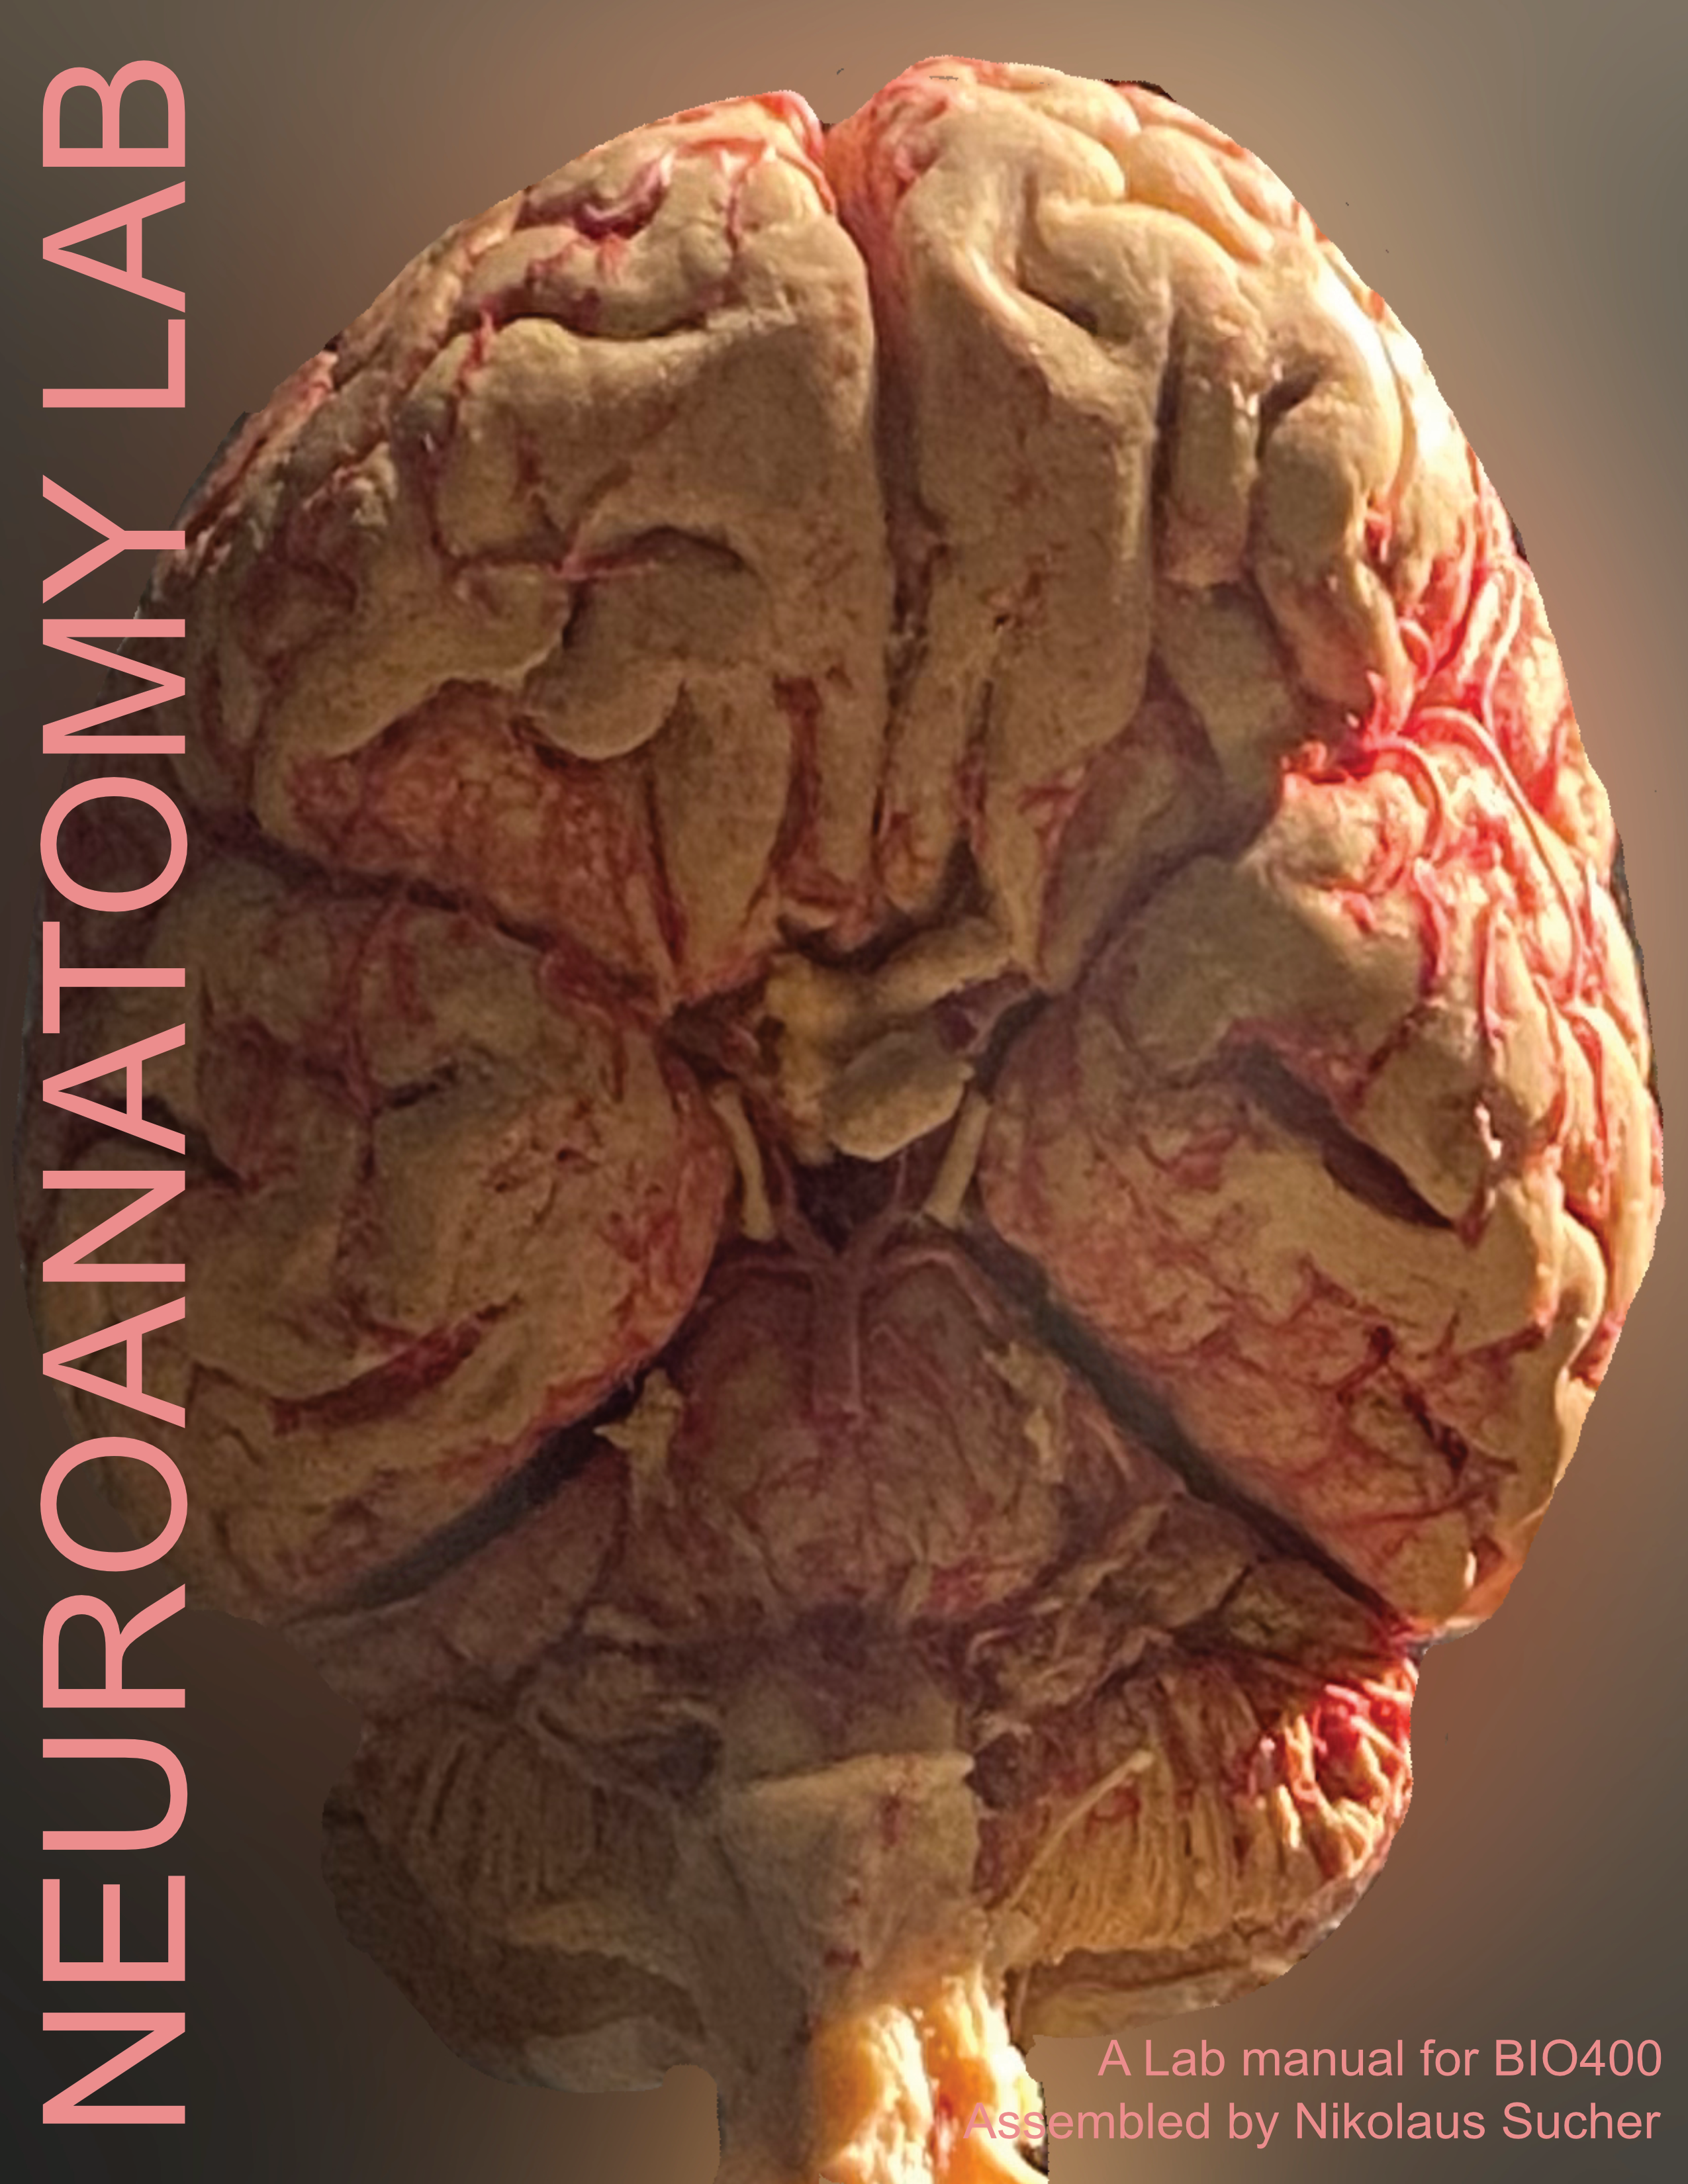
\includegraphics[width=0.7\linewidth]{neuroanatomy_lab_brain_cover} \end{center}

This work is licensed under the \href{https://creativecommons.org/licenses/by-sa/3.0/deed.en}{Creative Commons Attribution-Share Alike 3.0 Unported} United States License.

\hypertarget{acknowledgements}{%
\chapter*{Acknowledgements}\label{acknowledgements}}
\addcontentsline{toc}{chapter}{Acknowledgements}

The creation of this laboratory manual was greatly facilitated and owes a major debt to \href{https://www.wikipedia.org}{Wikipedia} and its large number of voluntary contributors. I very liberally copied from many Wikipedia pages and then remixed, edited, adapted and added text. With your continued support and help this book can only get better over time. I urge you to email me with your criticisms and suggestions at \href{mailto:nsucher@salemstate.edu}{\nolinkurl{nsucher@salemstate.edu}} This book is made available as an open educational resource under \href{https://creativecommons.org/licenses/by-sa/3.0/deed.en}{Creative Commons Attribution-Share Alike 3.0 Unported} United States License for others to do as I did and improve and adapt to specific requirements. I am grateful for the support provided by the Salem State University's OER initiative.

\hypertarget{surface-anatomy-of-the-brain}{%
\chapter{Surface Anatomy Of The Brain}\label{surface-anatomy-of-the-brain}}

In this laboratory session, we will study the surface anatomy of the human brain. Below, you will be presented with a number of figures and asked to label or color certain structures in each figure.

\hypertarget{a-dorsal-view-of-a-human-brain.}{%
\section{A dorsal view of a human brain.}\label{a-dorsal-view-of-a-human-brain.}}

\begin{enumerate}
\def\labelenumi{\arabic{enumi}.}
\tightlist
\item
  Write ``LH`` over the left hemisphere and ``RH`` over the right
hemisphere in figure 1 below.
\item
  Write ``ANTERIOR' and ``POSTERIOR`` next to the arrowhead pointing
in the corresponding direction: 

\item
  Mark the longitudinal cerebral fissure with a sequence of ``x'''s

\end{enumerate}



\begin{figure}

{\centering 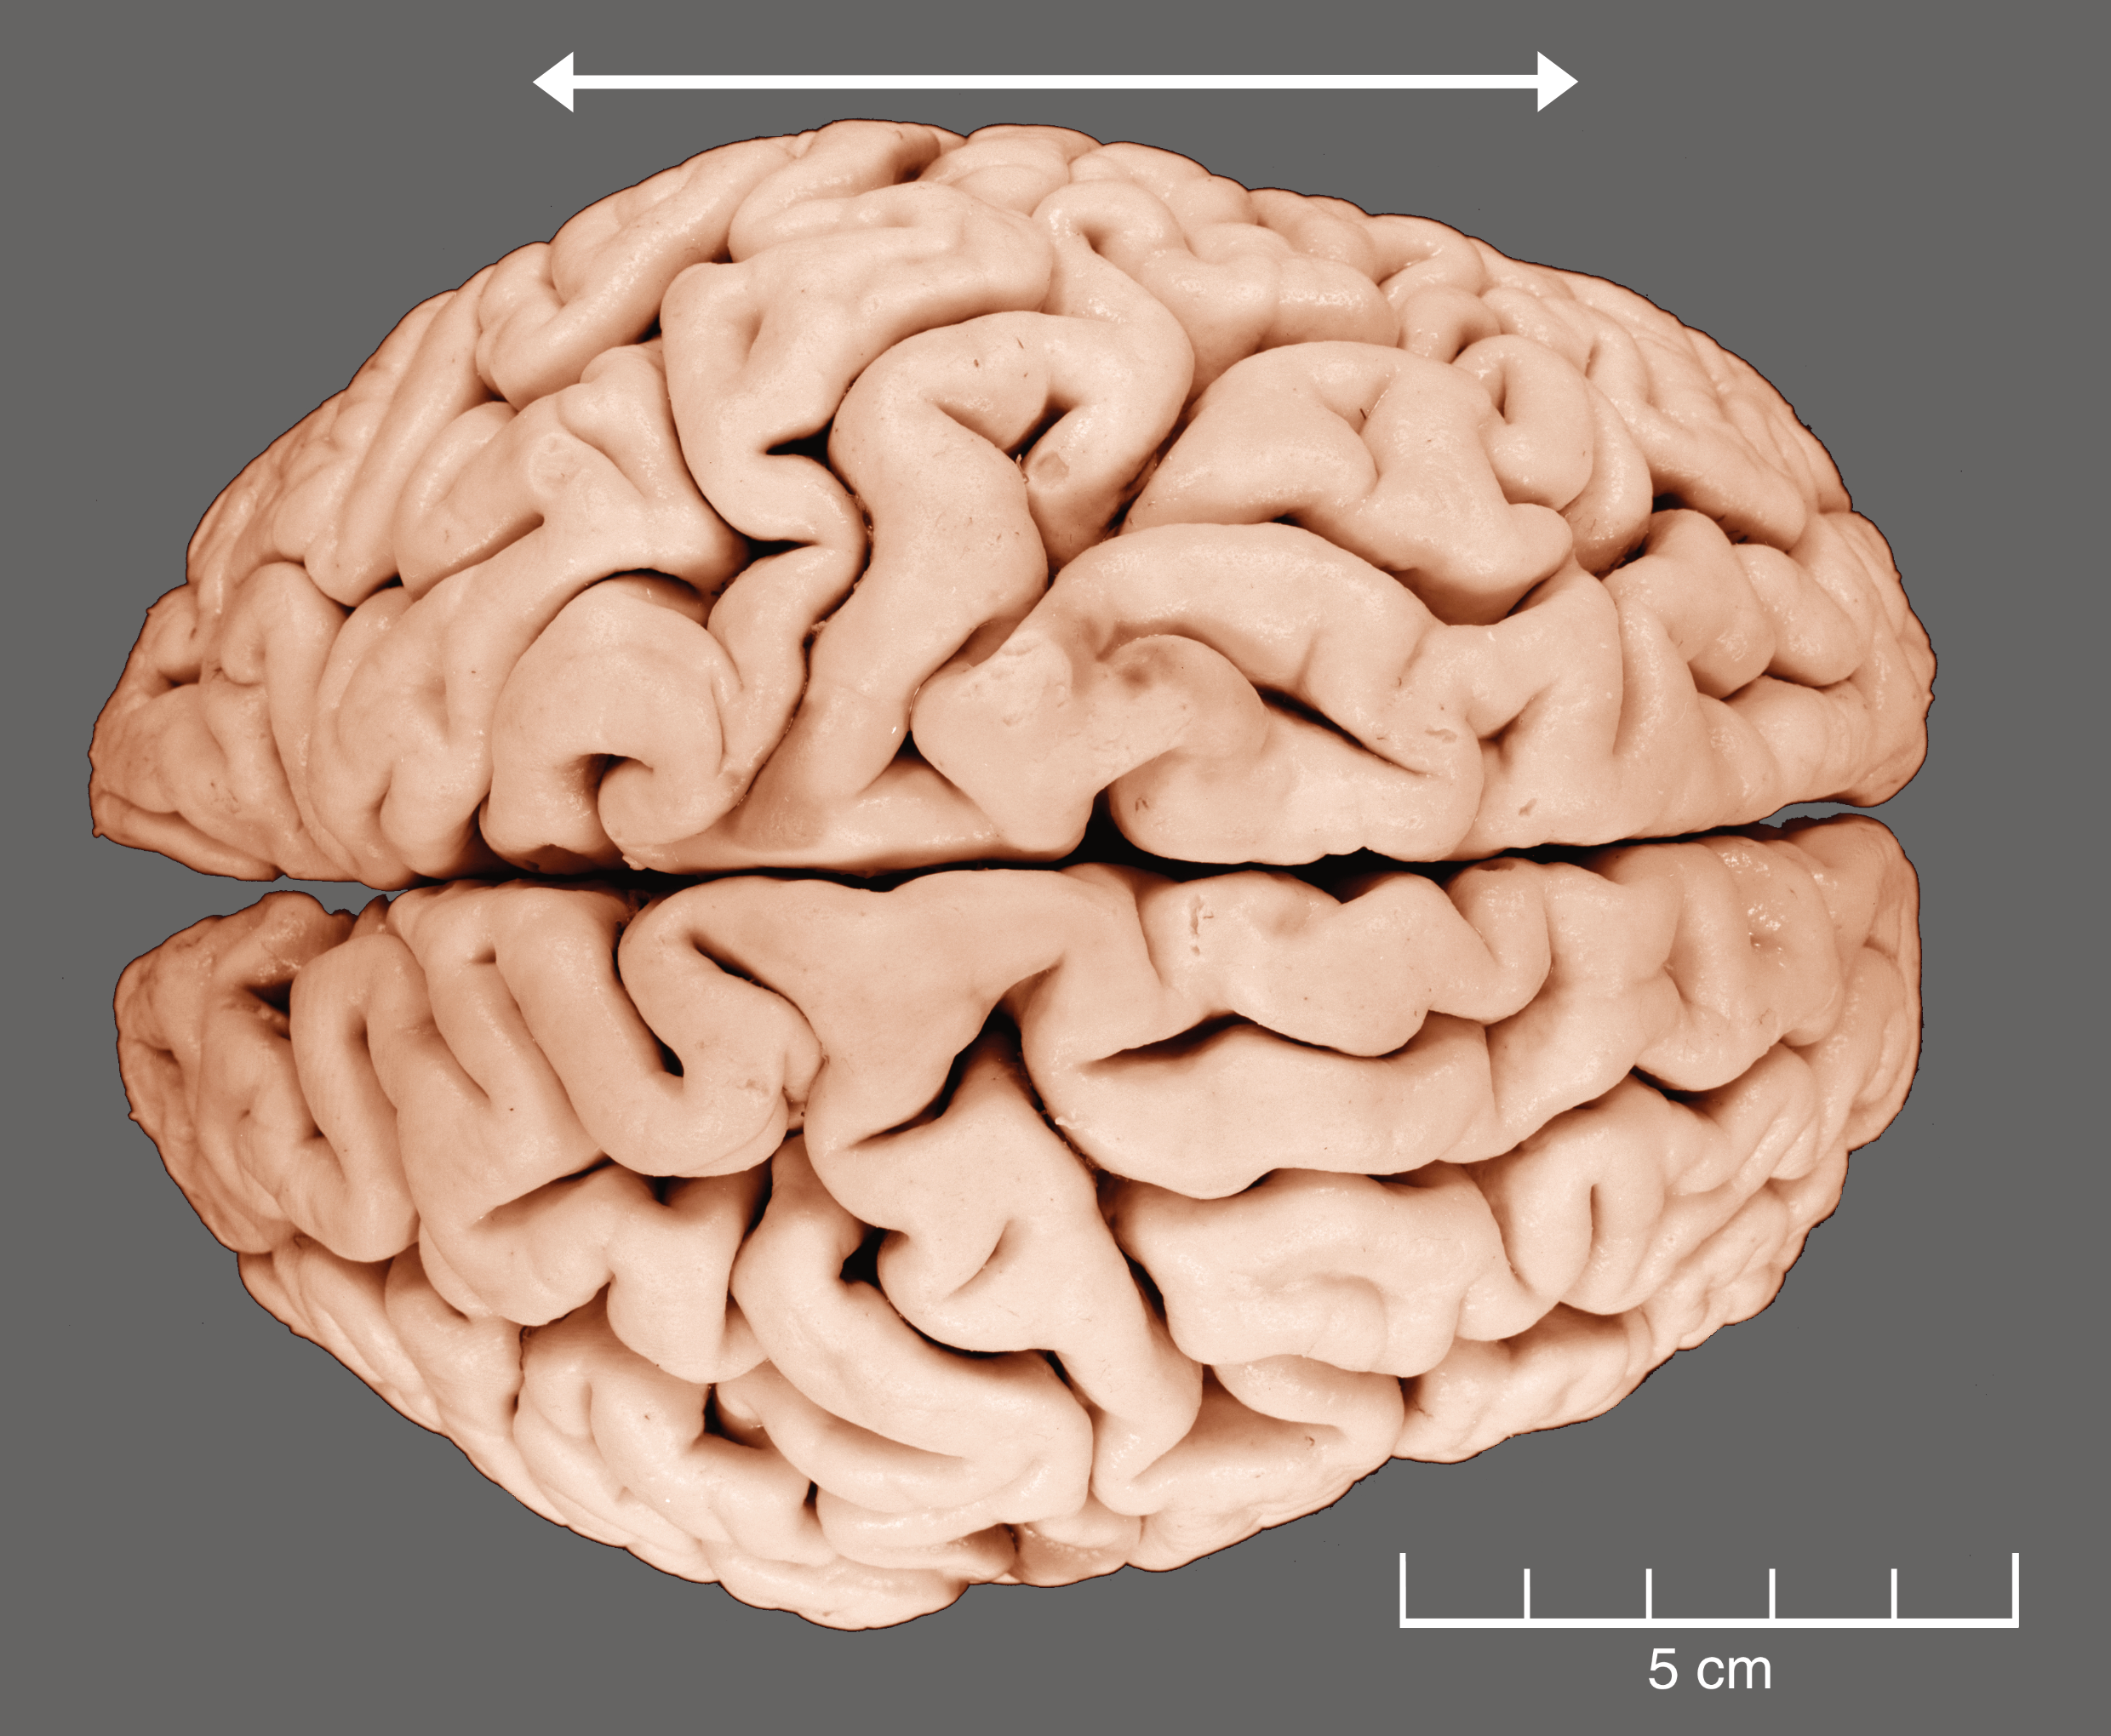
\includegraphics[width=0.7\linewidth]{./figures/cns/human_brain_dorsal} 

}

\caption{A dorsal view of a human brain.}\label{fig:hbdorsal}
\end{figure}

\hypertarget{a-dorso-lateral-view-of-a-human-brain.}{%
\section{A dorso-lateral view of a human brain.}\label{a-dorso-lateral-view-of-a-human-brain.}}

\begin{enumerate}
\def\labelenumi{\arabic{enumi}.}
\tightlist
\item
  Write ``ANTERIOR' and ``POSTERIOR`` next to the arrowhead pointing
in the corresponding direction 

\item
  Trace the Sylvian fissure using a black marker
\item
  Trace the central sulcus from the midline to the Sylvian fissure using a black marker
\end{enumerate}



\begin{figure}

{\centering 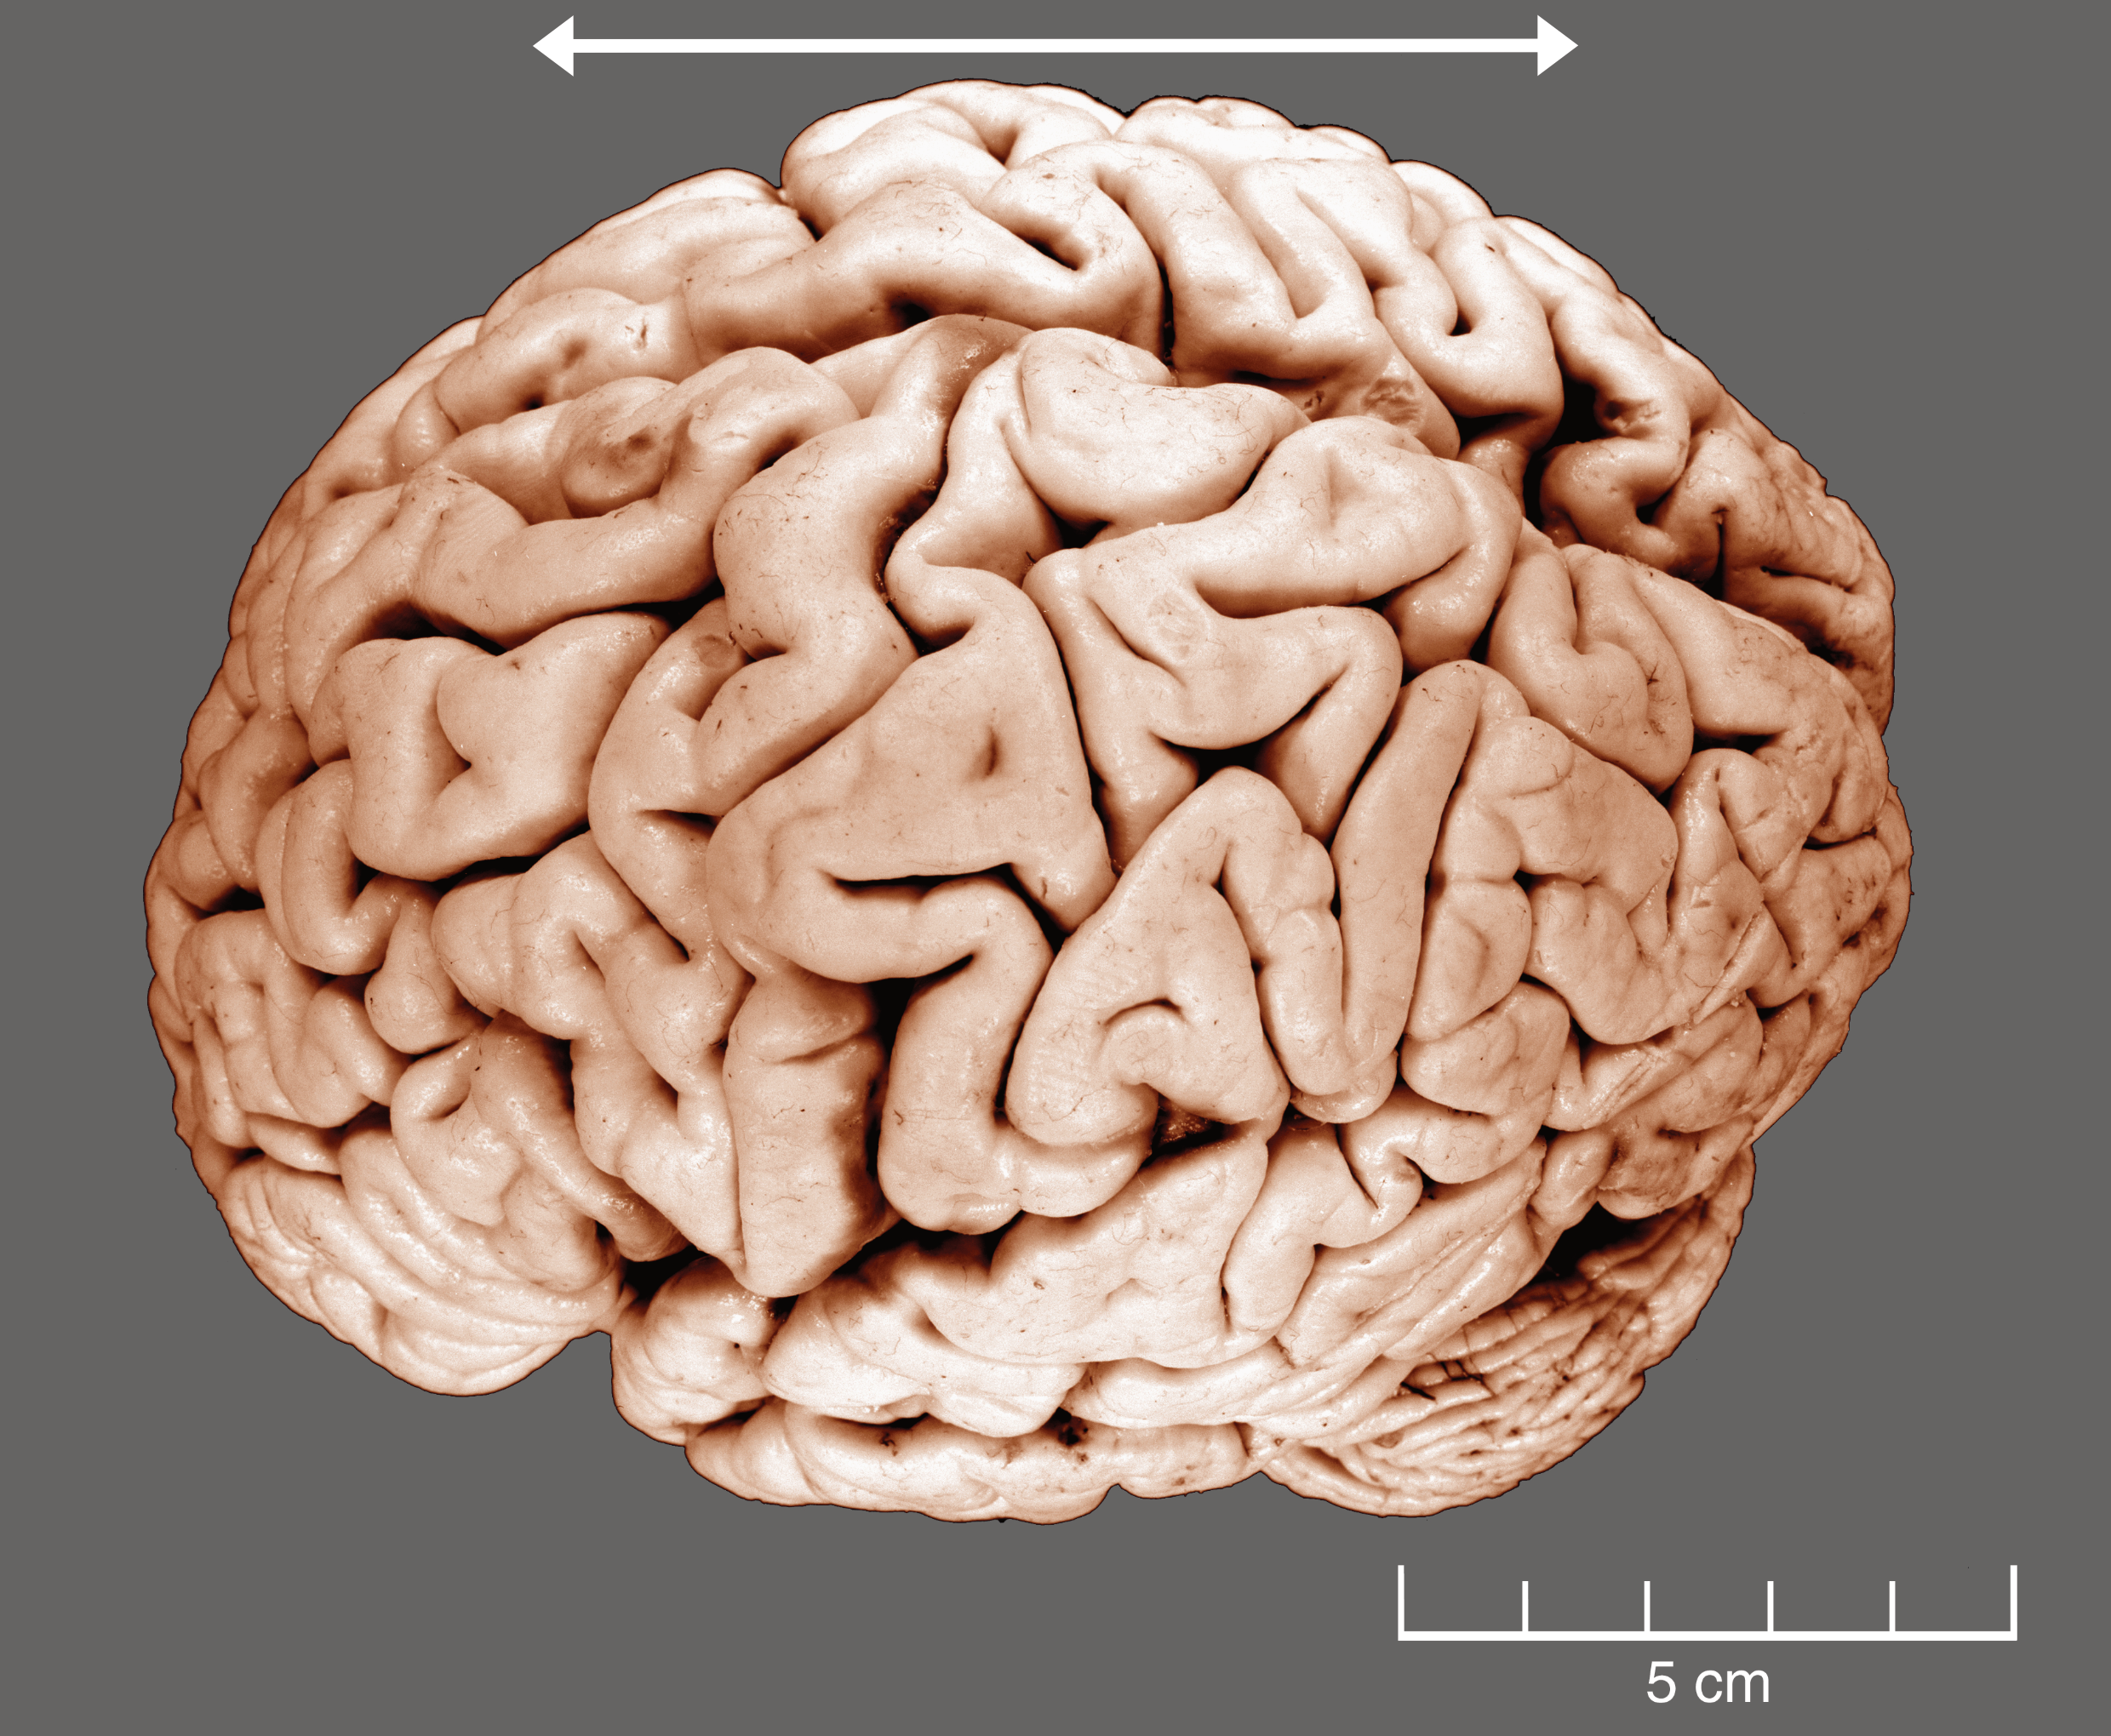
\includegraphics[width=0.7\linewidth]{./figures/cns/human_brain_dorsal_lateral} 

}

\caption{A dorso-lateral view of a human brain.}\label{fig:hbdl}
\end{figure}

\hypertarget{a-lateral-view-of-a-human-brain.}{%
\section{A lateral view of a human brain.}\label{a-lateral-view-of-a-human-brain.}}

\begin{enumerate}
\def\labelenumi{\arabic{enumi}.}
\tightlist
\item
  Write ``ANTERIOR' and ``POSTERIOR`` next to the arrowhead pointing
in the corresponding direction 

\item
  Write ``DORSAL`` and ``VENTRAL`` next to the arrowhead pointing
in the corresponding direction 

\item
  Write ``CEREBRUM`` and ``CEREBELLUM`` next to the corresponding structures
\item
  rite ``BRAINSTEM`` next to the corresponding structure

\item
  Write ``OLFACTORY BULB`` next to the corresponding structure

\end{enumerate}



\begin{figure}

{\centering \includegraphics[width=0.7\linewidth]{./figures/cns/human_brain_lateral} 

}

\caption{A lateral view of a human brain.}\label{fig:hbl}
\end{figure}

\hypertarget{a-ventral-view-of-a-human-brain.}{%
\section{A ventral view of a human brain.}\label{a-ventral-view-of-a-human-brain.}}

\begin{enumerate}
\def\labelenumi{\arabic{enumi}.}
\tightlist
\item
  Write ``LH`` over the left hemisphere and ``RH` over the right
hemisphere in figure 1 below.
\item
  Write ``LCblH`` over the left hemisphere of the cerebellum
and ``RCblH` over the right cerebellar hemisphere in the figure below.
\item
  Write ``Pons`` over the corresponding structure in the figure below.
\item
  Write ``MO`` denoting the medulla oblongata over the corresponding
structure in the figure below.
\item
  Write ``ANTERIOR' and ``POSTERIOR`` next to the arrowhead pointing
in the corresponding direction.

\end{enumerate}



\begin{figure}

{\centering 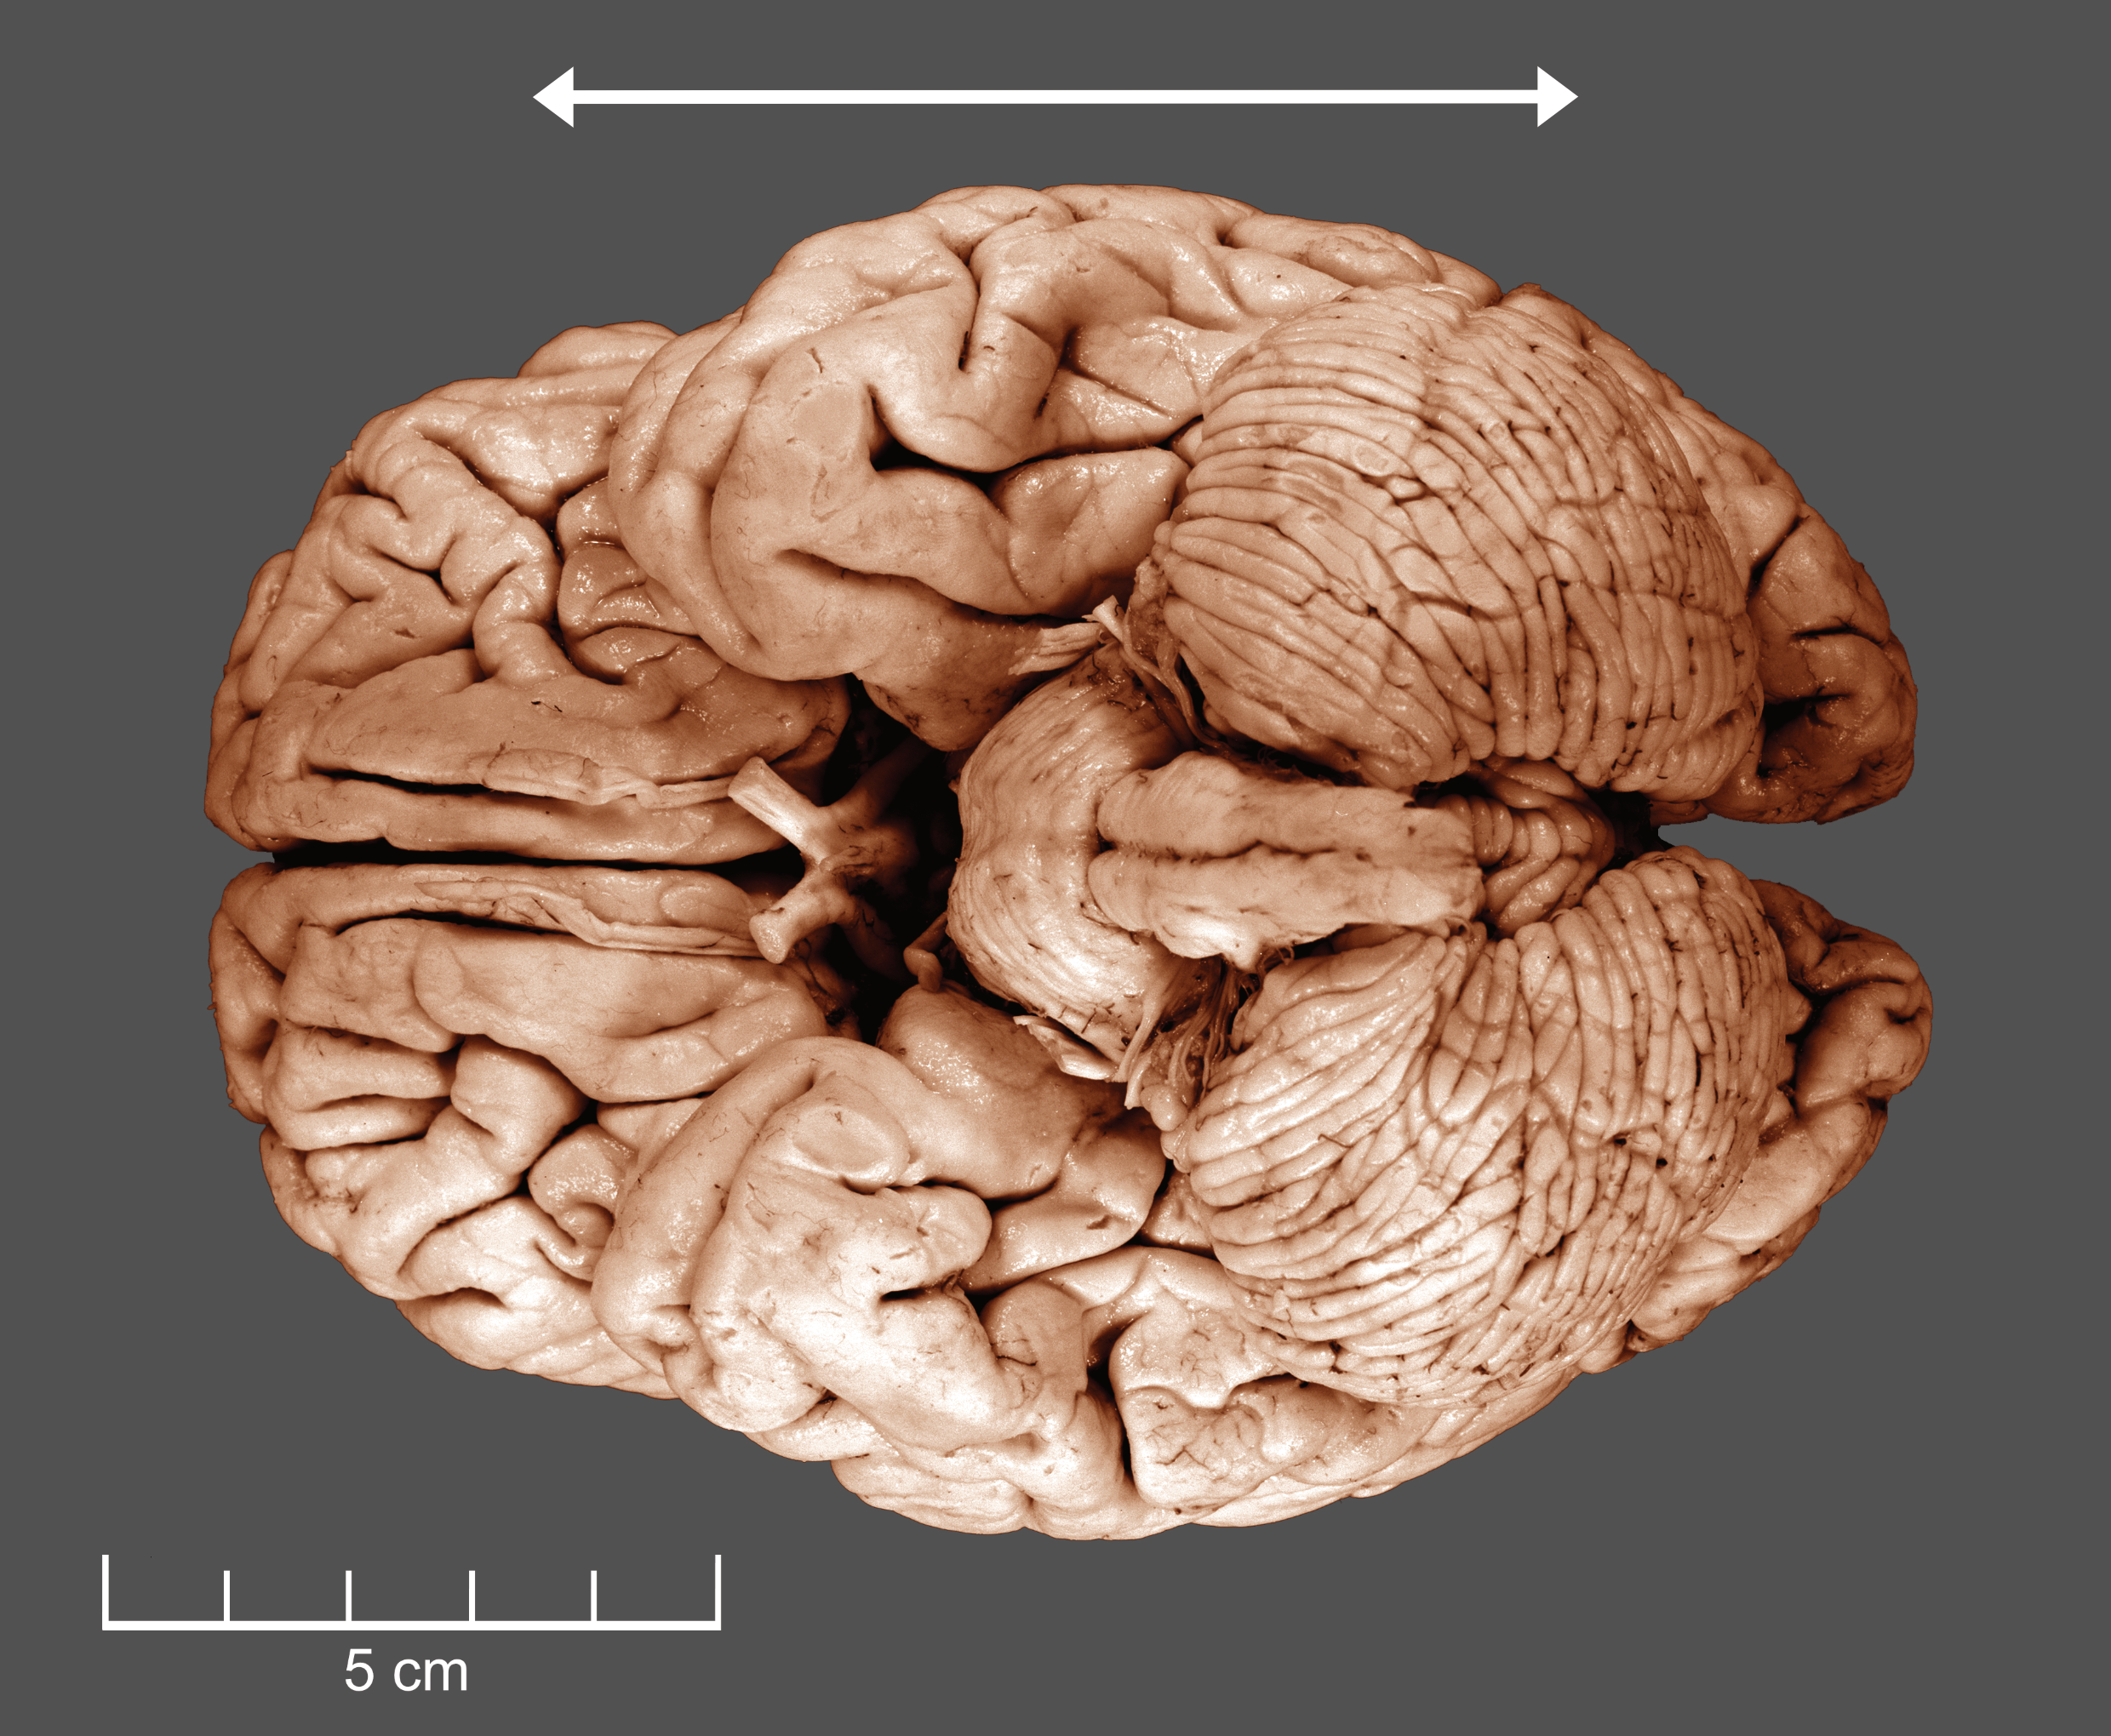
\includegraphics[width=0.7\linewidth]{./figures/cns/human_brain_ventral} 

}

\caption{A ventral view of a human brain.}\label{fig:hbv}
\end{figure}

\hypertarget{a-lateral-view-of-the-human-brain.}{%
\section{A lateral view of the human brain.}\label{a-lateral-view-of-the-human-brain.}}

\begin{enumerate}
\def\labelenumi{\arabic{enumi}.}
\tightlist
\item
  Color the frontal lobe red
\item
  Color the temporal lobe green
\item
  Color the parietal lobe yellow
\item
  Color the occipital lobe blue
\item
  Mark the central sulcus with a sequence of ``o``'s
\item
  Mark the Sylvian fissure with a sequence of ``x'''s

\end{enumerate}



\begin{figure}

{\centering \includegraphics[width=0.7\linewidth]{./figures/cns/brain_for_labeling_lobes} 

}

\caption{A lateral view of the major lobes of the human brain.}\label{fig:bfll}
\end{figure}

\begin{enumerate}
\def\labelenumi{\arabic{enumi}.}
\tightlist
\item
  Mark the central sulcus with a sequence of ``o``'s.
\item
  Mark the Sylvian fissure with a sequence of ``x'''s.
\item
  Color the precentral gyrus red.
\item
  Color the postcentral gyrus green.
\item
  Color the superior temporal gyrus blue.

\end{enumerate}



\begin{figure}

{\centering \includegraphics[width=0.7\linewidth]{./figures/cns/brain_for_labeling_gyri} 

}

\caption{A lateral view of the major gyri of the human brain.}\label{fig:bflg}
\end{figure}

\hypertarget{a-medial-view-of-the-human-brain.}{%
\section{A medial view of the human brain.}\label{a-medial-view-of-the-human-brain.}}

\begin{enumerate}
\def\labelenumi{\arabic{enumi}.}
\tightlist
\item
  Color the septum pellucidum yellow
\item
  Color the thalamus blue
\item
  Color the hypothalamus grey
\item
  Color the pons red
\item
  Color the medulla oblongata green
\item
  Color the tectum yellow
\item
  Color the tegmentum grey
\item
  Color the pineal body red

\end{enumerate}



\begin{figure}

{\centering \includegraphics[width=0.7\linewidth]{./figures/cns/brain_for_labeling_medial_I} 

}

\caption{A medial view of the human brain.}\label{fig:bflm}
\end{figure}

\begin{enumerate}
\def\labelenumi{\arabic{enumi}.}
\tightlist
\item
  Color the cingulate gyrus green
\item
  Color the corpus callosum red
\item
  Color the fornix yellow
\item
  Color the olfactory bulb blue
\item
  Color the optic chiasm grey

\end{enumerate}



\begin{figure}

{\centering \includegraphics[width=0.7\linewidth]{./figures/cns/brain_for_labeling_medial_II} 

}

\caption{A medial view of a human brain.}\label{fig:bflmii}
\end{figure}

\begin{enumerate}
\def\labelenumi{\arabic{enumi}.}
\tightlist
\item
  Color the third ventricle green
\item
  Color the aqueduct red
\item
  Color the fourth ventricle blue
\item
  Color the spinal call yellow

\end{enumerate}

A medial view of a human brain. A medial view of a human brain.

\begin{figure}

{\centering \includegraphics[width=0.7\linewidth]{./figures/cns/brain_for_labeling_medial_III} 

}

\caption{(ref:blmiii)}\label{fig:bflmiii}
\end{figure}

\hypertarget{cytoarchitectonic-areas-according-to-brodmann}{%
\section{Cytoarchitectonic areas according to Brodmann}\label{cytoarchitectonic-areas-according-to-brodmann}}

\begin{enumerate}
\def\labelenumi{\arabic{enumi}.}
\tightlist
\item
  Label the highlighted areas with the corresponding numbers given by Broadmann.
\end{enumerate}



\begin{figure}

{\centering \includegraphics[width=0.7\linewidth]{./figures/cns/Brodmann_lateral} 

}

\caption{A lateral view of the cytoarchitectonic areas of the human brain according to Brodmann.}\label{fig:brodl}
\end{figure}

\begin{enumerate}
\def\labelenumi{\arabic{enumi}.}
\tightlist
\item
  Label the highlighted Brodamann areas with the corresponding numbers.
  (ref:bm) A medial view of the cytoarchitectonic areas of the human brain according to Brodmann
\end{enumerate}

\begin{figure}

{\centering \includegraphics[width=0.7\linewidth]{./figures/cns/Brodmann_medial} 

}

\caption{(ref:bm)}\label{fig:brodm}
\end{figure}


\end{document}
